\documentclass[10pt]{article}
\usepackage[a4paper,margin=2cm]{geometry}
\usepackage{graphicx}
\usepackage{microtype}
\usepackage{booktabs}
\usepackage{float}
\usepackage[hidelinks]{hyperref}
\usepackage{parskip}
\setlength{\parskip}{4pt}

\begin{document}

{\LARGE\bfseries The energy allometry of settlements}

\vspace{2pt}
{\large Working title --- prospectus for discussion, August 2026}

\section*{Abstract}

In organisms, energy use rises more slowly than size, because a larger body is
served by proportionally more shared structure. Settlements built before the
car obeyed the same law, since everyday reach on foot required compact fabric
at every settlement size; development since has escaped it by spending energy
instead. We test both claims with metered gas and electricity for 178,353
English neighbourhoods, car-travel energy anchored to the National Travel
Survey, and each neighbourhood's build year. Fabric with a median build year
before 1919 remains 55 per cent flats and terraces from market town to
metropolis, and its total energy rises sublinearly with settlement size, at an
exponent of 0.94 (95 per cent confidence interval 0.93 to 0.95). Fabric of the
motor decades falls to a third compact and scales one-for-one with size, at
1.02 (0.97 to 1.06), while its residents reach much the same destinations by
driving across larger catchments. A wholly detached neighbourhood uses about
twice the energy of a wholly flat one for much the same reach by car, and
population size now explains five per cent of the variation in built form.
Priced against each district's own fabric at its inherited compactness, the
compensation comes to 20 terawatt-hours a year, with the dispersed shires ten
per cent above their benchmark and the largest cities at or below theirs. The
economy of scale that organisms collect through size remains open to
settlements through form, and dispersed growth is the continuing choice to
leave it uncollected.

\section*{The argument in four steps}

\textbf{1. The principle is a law of energy.} Ecology's allometric laws were
laws of energy before urban scaling borrowed the term: metabolic rate rises as
roughly the three-quarter power of body mass, because shared distribution
structure serves a larger body more efficiently (Kleiber 1932; West, Brown and
Enquist 1997). Jane Jacobs stated the urban counterpart as energy
productivity: a system with more structure extracts more use from the same
unit of energy. A companion paper measures that productivity directly, and
compact neighbourhoods obtain about four times the everyday access per
kilowatt-hour of dispersed ones.

\textbf{2. Historic settlements follow the law.} Neighbourhoods whose fabric
predates 1919 are 55 per cent flats and terraces whatever the size of the
settlement, because reach on foot constrained every town alike
(Fig.~\ref{fig:era}). The energy of that fabric carries the allometric
signature today: it rises sublinearly with settlement size, at an exponent of
0.94 (0.93 to 0.95), the direction Kleiber's law predicts.

\textbf{3. Modern development breaks the law by compensation.} Motorised
energy released the walking constraint, and the fabric of 1919 to 1979 fell to
about a third flats and terraces at every settlement size, while its energy
scales one-for-one with population (exponent 1.02, 0.97 to 1.06): the economy
of scale is gone from it. The compensation is measurable, because residents of
dispersed fabric reach much the same destinations counted at their own car
catchments and pay the difference in travel energy. Size and form have come
apart, with population size explaining five per cent of the variation in
compactness. Public transport is the release that keeps the law: a bus or
train dilates reach through shared structure at a fraction of the car's energy
per passenger-mile, where the car dilates it by multiplying private energy.

\textbf{4. The forgone economy, priced.} Re-pricing every neighbourhood built
since 1919 at the compactness its own district inherited, England would spend
about 20 terawatt-hours a year less on homes and car travel, four per cent of
the total. The burden is uneven (Fig.~\ref{fig:bloat}): the dispersed shire
districts sit about ten per cent above their inherited benchmark, while the
large cities sit at or below theirs. The law is also recoverable, because
fabric built since 1980 re-couples with size (exponent 0.95, 0.91 to 1.00)
through flat-led building in the largest cities.

\newpage

\begin{figure}[H]
\centering
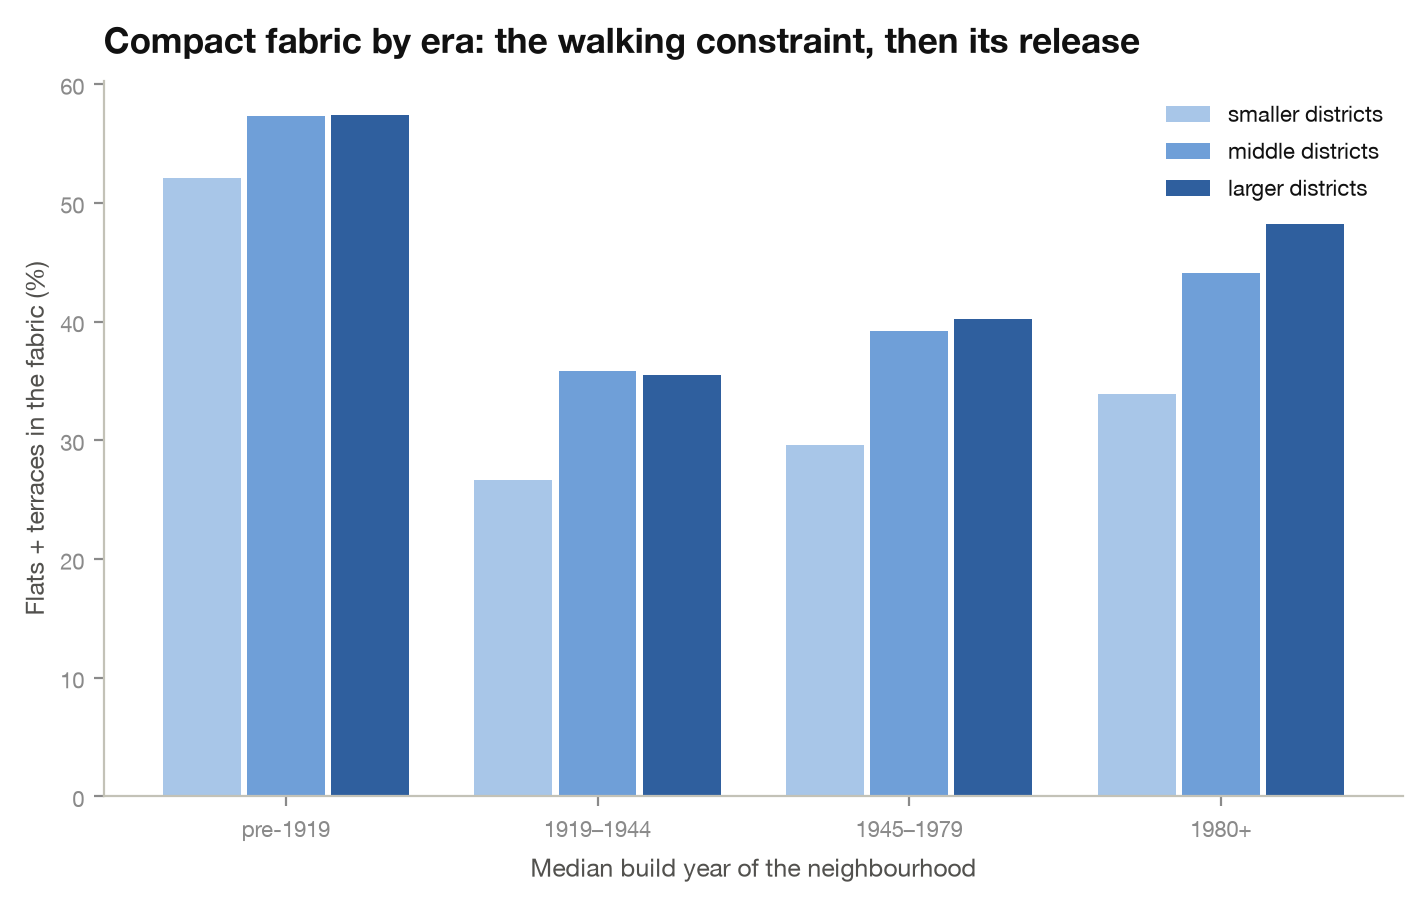
\includegraphics[width=0.72\textwidth]{fig_era.png}
\caption{Flats and terraces as a share of each era's fabric, by settlement-size
tercile. Pre-1919 fabric is compact at every size; the motor decades fall to
about a third; fabric since 1980 recovers a size gradient.}
\label{fig:era}
\end{figure}

\begin{figure}[H]
\centering
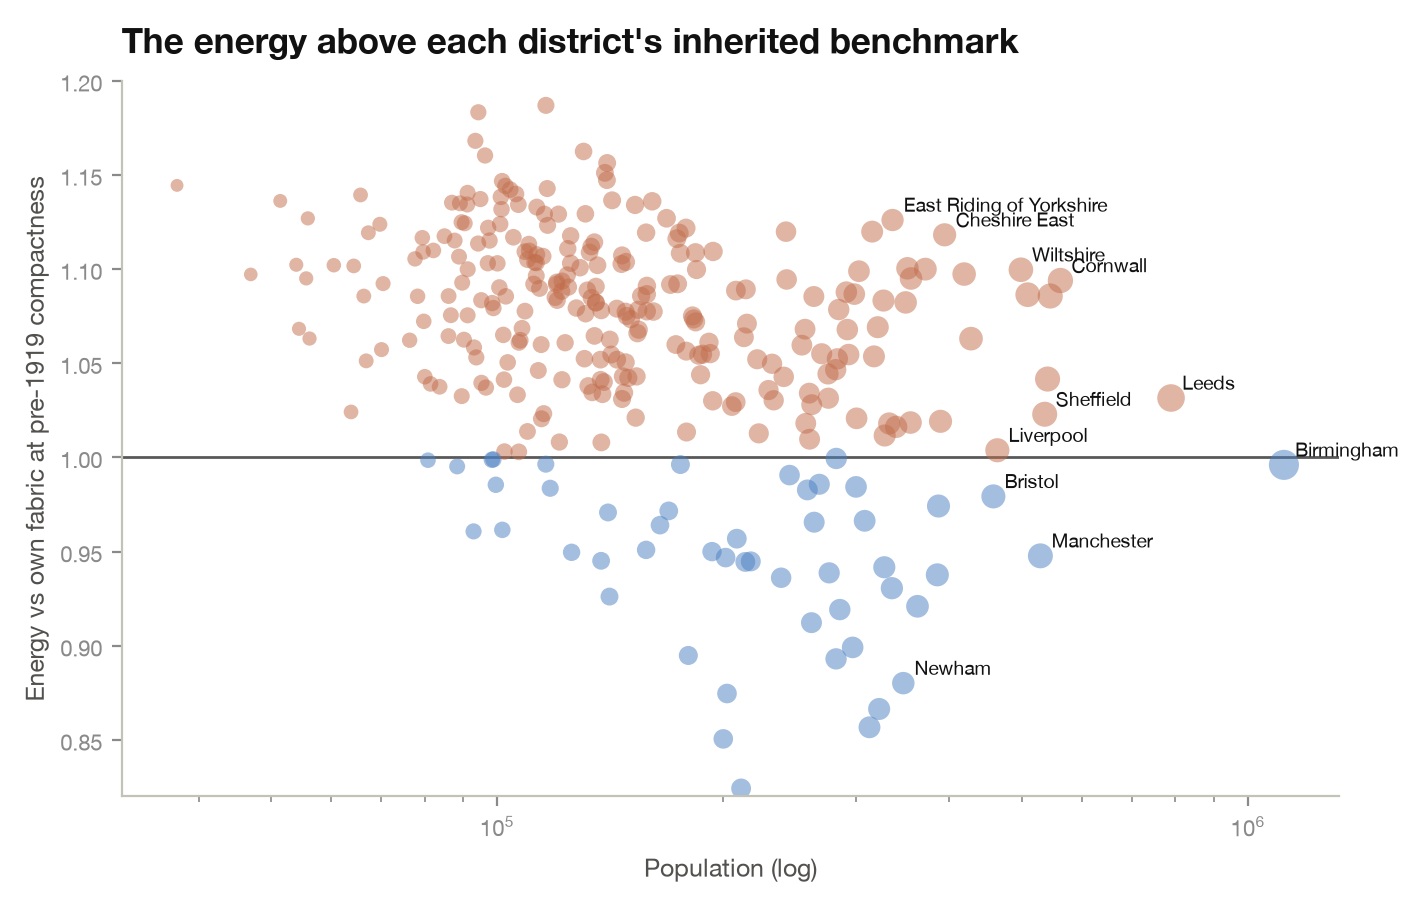
\includegraphics[width=0.72\textwidth]{fig_bloat.png}
\caption{Each district's observed energy against its own fabric re-priced at
pre-1919 compactness. Districts above the line pay for dispersion in energy;
districts below out-collect their inherited benchmark.}
\label{fig:bloat}
\end{figure}

\section*{Data and status}

Pilot estimates, computed from open data already assembled for the companion
paper: metered gas and electricity (DESNZ, postcode level), Census 2021
dwelling-type composition and build year (EPC medians), and car-travel energy
disaggregated from National Travel Survey mileage by settlement class. Home
energy is metered; travel is a survey-anchored construction, and the clean
metered exponent is reported alongside every travel-inclusive one. The pilot
uses local authority districts as the settlement unit; the paper would
re-estimate on ONS Built-Up Areas, add the public-transport bound, and carry
the confound set of the companion paper (build year, deprivation, tenure,
climate) through every fit. Companion: \emph{the lock-in manuscript} (in
preparation), which supplies the two-times energy gap, the equal-reach
catchment result, and the access-per-kilowatt-hour rate cited above.

\end{document}
